\documentclass[a4paper, openany, oneside]{memoir}
\usepackage[T1]{fontenc}
\usepackage{lmodern}
\usepackage[utf8]{inputenc}
\usepackage[german]{babel}
\usepackage[obeyspaces, hyphens]{url}
\usepackage{graphicx}
\usepackage{listings}
\usepackage{color}
\usepackage{siunitx}
\usepackage{tabularx}
\usepackage{hyperref}

\graphicspath{{./img/}}

\pretitle{\begin{center}\Huge\bfseries}
\title{User Guide für das Erstellen von Druckstatistiken}
\posttitle{\par\vskip1em{\normalfont\normalsize In Bezug zu Abdrücken von Klauen auf Tekscan-Druck-Sensoren\par\vfill}\end{center}}
\author{Kai Hainke}
\predate{\vfill\begin{center}\large}
\chapterstyle{thatcher}

\DeclareUrlCommand{\dir_path}{\def\UrlLeft{\textrm{»}}\def\UrlRight{\textrm{«}}}

\DeclareUrlCommand{\File_path}{\def\UrlLeft{\textrm{}}\def\UrlRight{\textrm{}}}

\DeclareUrlCommand{\file_ending}{\def\UrlLeft{\textrm{}}\def\UrlRight{\textrm{}}}


\definecolor{dkgreen}{rgb}{0,0.6,0}
\definecolor{gray}{rgb}{0.5,0.5,0.5}
\definecolor{mauve}{rgb}{0.58,0,0.82}
\lstset{frame=tb,
  language=Python,
  aboveskip=3mm,
  belowskip=3mm,
  showstringspaces=false,
  columns=flexible,
  basicstyle={\small\ttfamily},
  numbers=none,
  numberstyle=\tiny\color{gray},
  keywordstyle=\color{blue},
  commentstyle=\color{dkgreen},
  stringstyle=\color{mauve},
  breaklines=true,
  tabsize=3
}



\begin{document}


\maketitle


%\pagebreak
%\dirpath{Documents\BliBla\bludsdus\dssdsd}\linebreak\linebreak
%\url{Documents\BliBla\bludsdus\dssdsd}
%\pagebreak


\chapter{Voraussetzungen}
\section{Tools}
In diesem Guide werden folgende Tools benutzt:
\begin{enumerate}
\item Python 2.7.13 mit folgenden Paketen (zu installieren mit zBsp. pip install pyclipper):
\begin{enumerate}
\item numpy
\item pyclipper 
\item sklearn
\end{enumerate}
\item Maya 2014
\item ProKlaue Plugin 0.3.4
\item XROMM Plugin
\item R für Plots
\end{enumerate}

\section{Verzeichnisstruktur}
Das Basisverzeichnis für diesen Guide ist \\\dir_path{Documents\ProKlaue\testdaten\druck}.\\
Darunter sollte pro Klaue ein Ordner der Form  \\\dir_path{Klaue <Nr.> (K<Nr.>T)} liegen.\\ In diesem Ordner wiederum sollten alle benötigten Dateien zur Klaue liegen und auch dorthin geschrieben werden.

\section{Ausgangsdateien}
Zusätzlich müssen folgende Dateien vorliegen (jeweils pro Klaue, im Ordner der Klaue):
\begin{enumerate}
\item Jeweils für links und rechts 1 \file_ending{.obj}-Datei 
\item 1 Ordner mit rigid-body-matrix-Dateien für das XROMM Plugin, dieser sollte jeweils für links und rechts mind. 1 \file_ending{.csv}-Datei enthalten
\item 1 Tekscan \file_ending{.csv}-Datei mit Daten von den Drucksensoren 
\item 2 Definitionen von Messzonen für die Statistik, siehe \ref{zone_def}
\item das \File_path{pressureStatistics.py} - Script zusammen mit dem\\ \File_path{pressureStatisticsUtilFunctions.py} Script
\end{enumerate}

\section{Variablen}
Der Nutzer muss außerdem den Wert für folgende Variablen festlegen:
\begin{enumerate}
\item Einsinktiefe a.k.a. der Höhen-Wert für den der Abdruck des Oberflächennetzes der Klaue bestimmt wird \label{th_def}
\item Zonenraster, Definition der Zonen für die Statistik, diese sollten in relativen Koordinaten definiert werden (\((0,0)\) ist der untere linke Punkt der Klaue in Ausrichtung vorne-hinten(\(\leftarrow x\rightarrow\)), Links-Rechts (\(\leftarrow y\rightarrow\)), \((1,1)\) der obere rechte). In den Standard-Dateien (\File_path{Documents\ProKlaue\testdaten\druck\segments_for_measurements_<side>.csv}) sind die Zonen definiert wie in Abbildung \ref{img_zones}. \label{zone_def} Diese Dateien sollten auch im Basis-Verzeichnis liegen und dementsprechend benannt sein.
\end{enumerate}


\begin{figure}
\begin{center}
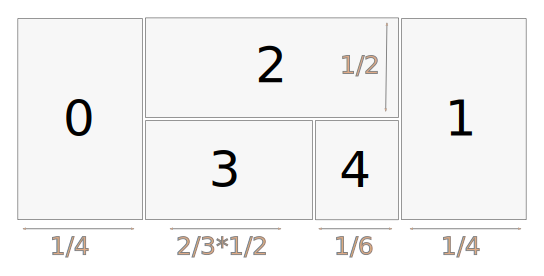
\includegraphics[width = 0.7\textwidth,keepaspectratio]{zones.eps}
\end{center}
\caption{Standard Messzonen (rechte Klaue)}
\label{img_zones}
\end{figure}

\chapter{Workflow}
\begin{figure}
\begin{center}
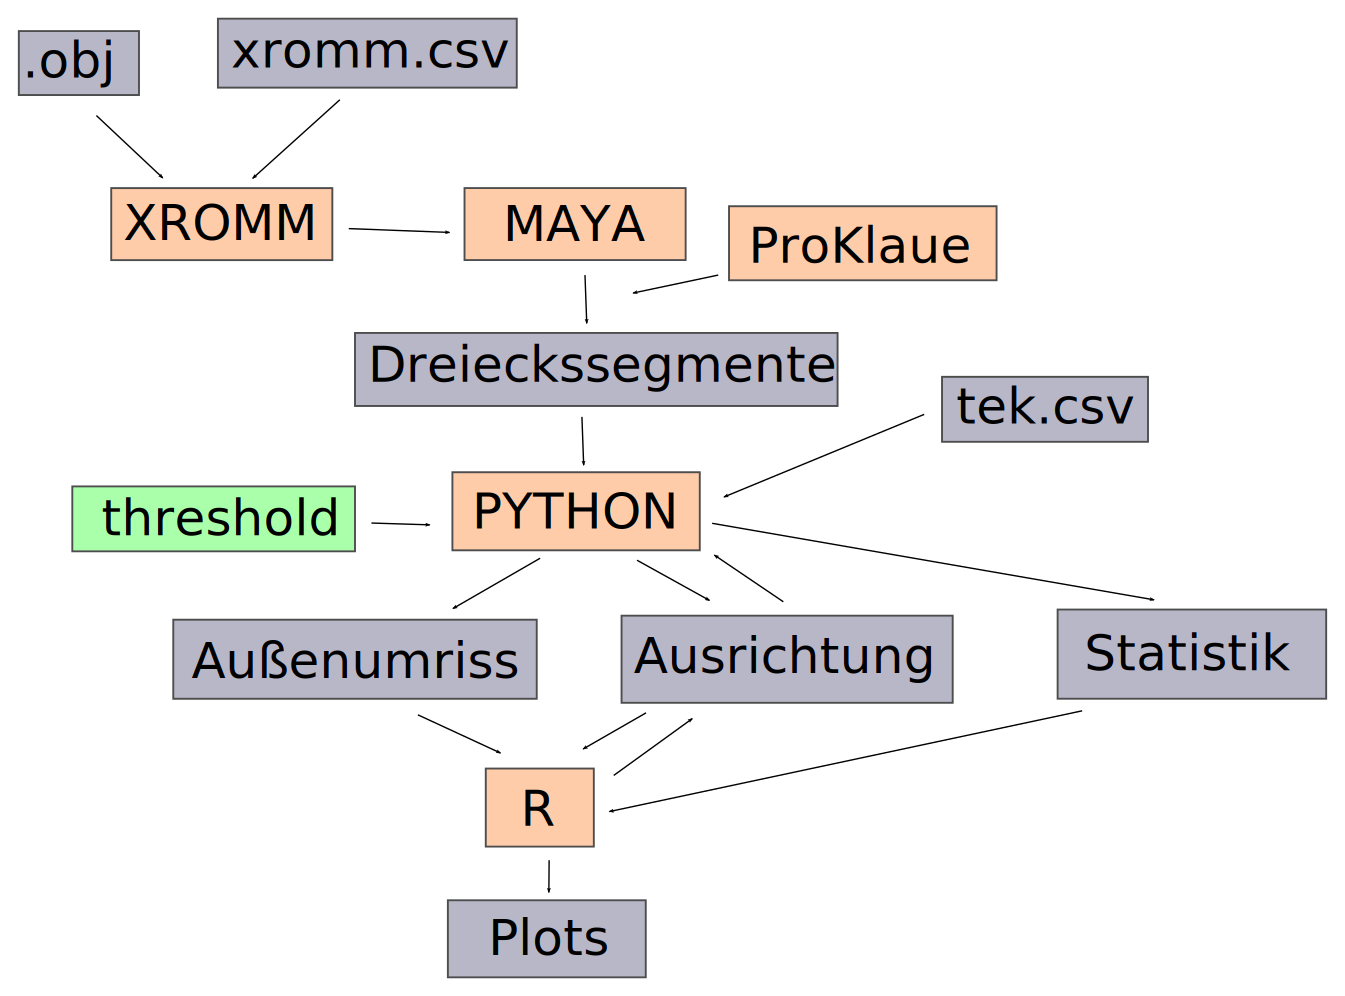
\includegraphics[width = 0.7\textwidth,keepaspectratio]{workflow.eps}
\end{center}
\caption{allgemeiner Workflow}
\label{img_workflow}
\end{figure}
Zunächst wird aus den Dateien für das XROMM-Plugin das Modell der Klaue in Maya eingeladen. Danach wird hierfür eine Liste von Dreieckssegmenten des Oberflächenmodells errechnet. Mittels eines Thresholds und Clipping wird durch Python ein Außenumriss errechnet. Außerdem wird eine vorläufige Transformation zur Ausrichtung an den Druckdaten errechnet. Mittels R lässt sich dies darstellen und ggf. anpassen. Nach einer erneuten Berechnung durch Python lässt sich dann auch die Statistik zu den Zonen verwerten.
\section{Erstellen des Außenumriss}
Zunächst ruft man das Import-XROMM-Plugin in Maya auf. Dann importiert man durch Klick auf den Button impObjs die entsprechenden \file_ending{.obj}-Dateien der Klauen (in diesem Fall erst links, dann rechts, den Dialog zum Skalieren mit Yes bestätigen). Dann wählt man die entsprechenden \file_ending{.csv}-Dateien mit den rigid-body-Koordinaten, hier wieder erst links dann rechts. Dann wählt man im Outliner die eben importierten Objekte aus (links, dann rechts). Dann die Option Rigid Body Matrix im Data type Reiter anklicken und den Haken bei Coloumn Headers in Row entfernen. Zuletzt auf import klicken. Siehe Abb. \ref{img_xromm_options}.

\begin{figure}
\begin{center}
\includegraphics[height = 0.5\textheight, width=1\textwidth,keepaspectratio]{xromm.png}
\end{center}
\caption{XROMM Optionen}
\label{img_xromm_options}
\end{figure}


Jetzt mithilfe des app Plugins (ProKlaue) eine achsenparallele Ebene erstellen für eine der beiden Klauen. Standardeinstellungen belassen und auf create klicken.

\begin{figure}
\begin{center}
\includegraphics[height = 0.2\textheight, width=1\textwidth,keepaspectratio]{app.png}
\end{center}
\caption{ProKlaue app}
\label{img_app}
\end{figure}


Nun jeweils eine Klaue und die Ebene auswählen und den folgenden Python-Befehl benutzen:

\begin{minipage}[c]{\textwidth}
\begin{lstlisting}[language=bash]
cmds.frontVertices(tsf="<>/Documents/ProKlaue/testdaten/druck/<Klauen-Verzeichnis>/tsf_<left oder right>.csv")
\end{lstlisting}
\end{minipage}


Stellen in Klammern \texttt{<>} sind zu ersetzen. Auch darauf achten, Pfade mit / und nicht mit \textbackslash{} zu schreiben.

\begin{figure}
\begin{center}
\includegraphics[height = 0.35\textheight, width=1\textwidth,keepaspectratio]{frontVertices.png}
\end{center}
\caption{ProKlaue frontVertices}
\label{img_frontVertices}
\end{figure}

Nun findet sich im Ordner der Klaue 2 neue Dateien \File_path{tsf_left.csv} und \File_path{tsf_left.csv}. Anschließend navigiert man zum \File_path{pressureStatistics.py} Script und führt es mit folgenden Parametern aus:


\begin{minipage}[c]{\textwidth}
\begin{lstlisting}[language=bash]
ProKlaue\scripts>python pressureStatistics.py -s <step> -t <threshold> -b "<klauenname>" -g "<bodentyp>" -d "<base_directory>"
\end{lstlisting}
\end{minipage}

th ist der Wert der Einsinktiefe (hier in cm), siehe \ref{th_def}. Der Wert für -b (bone) muss dem Namen des Klauen-Verzeichnis entsprechen. Und der Name des Boden (-g) sollte kleingeschrieben sein, die Beschriftung für die TEK-Dateien sollte jedoch den Namen großgeschrieben beinhalten. Wieder darauf achten, Pfade mit / und nicht mit \textbackslash{} zu schreiben.

Zunächst beginnt man mit step=0. 
\\\\
(OPTIONAL: Dabei sollte man den PYTHONPATH so anpassen, dass er auch das script modul findet. Dies macht man am besten unter Windows, Systemsteuerung, System und Sicherheit, System, Erweiterte Systemeinstellungen, Reiter Erweitert, Umgebungsvariablen, Reiter Systemvariablen, Neu, dann:\\
Name der Variable: \texttt{PYTHONPATH}\\
Wert der Variable: \texttt{<>\textbackslash Documents\textbackslash ProKlaue;<>\textbackslash Documents\textbackslash ProKlaue\textbackslash scripts}\\
Die Ordner so anpassen, dass das ProKlaue-Verzeichnis und das scripts Verzeichnis dort auftauchen, durch Semikolon getrennt. Bestätigen und Eingabeaufforderung öffnen.)\\
\\
Dann das Skript ausführen, siehe auch Abb. \ref{img_pressureStatistics_step0}:

\begin{minipage}[c]{\textwidth}
\begin{lstlisting}[language=bash]
C:\Users\Kai\Documents\ProKlaue\scripts>python pressureStatistics.py -s 0 -t 0.5 -b "Klaue 1 (K1T)" -g "gummi" -d "C:/Users/Kai/Documents/ProKlaue/testdaten/druck"
\end{lstlisting}
\end{minipage}


\begin{figure}
\begin{center}
\includegraphics[height = 0.5\textheight, width=1\textwidth,keepaspectratio]{script.png}
\end{center}
\caption{Ausführen des Python Skripts}
\label{img_pressureStatistics_step0}
\end{figure}

Danach findet man 2 Segment-Dateien für den Umriss im Klauen-Verzeichnis, diesen Schritt muss man nur einmal pro Klaue machen (Heißt man könnte auch hier weiter machen, falls man den 2ten Boden bearbeitet). Die nächsten Schritte müssen pro Boden ausgeführt werden. 

\begin{figure}
\begin{center}
\includegraphics[height = 0.5\textheight, width=1\textwidth,keepaspectratio]{klauenordner_1.png}
\end{center}
\caption{Klauenordner nach step=1}
\label{img_ordner_step1}
\end{figure}

Dann definiert man den Bodenparameter im Skript und setzt den Schrittparameter auf 1:


\begin{minipage}[c]{\textwidth}
\begin{lstlisting}[language=bash]
C:\Users\Kai\Documents\ProKlaue\scripts>python pressureStatistics.py -s 1 -t 0.5 -b "Klaue 1 (K1T)" -g "gummi" -d "C:/Users/Kai/Documents/ProKlaue/testdaten/druck"
\end{lstlisting}
\end{minipage}

Ausführen, man findet Dateien zur Transformationen und Druckdaten im Klauenverzeichnis. 



\section{Anpassen}

Nun kann man im R Skript (\File_path{scripts\druck.R}) mittels folgender Befehle die Transformation anpassen. Erst die Parameter im SETTINGS-Block anpassen, also Basisverzeichnis, Bodentyp (kleingeschrieben) und Klauen(verzeichnis)-Name angeben:

\begin{minipage}[c]{\textwidth}
\begin{lstlisting}[language=R]
setwd("~/ProKlaue/testdaten/druck")
ground_type = "beton"
bone = "Klaue 3 (K3T)"
\end{lstlisting}
\end{minipage}

Und nach Ausführen des SETTINGS-Code-Blocks und des TRANSFORM FIT - Code-Blocks lassen sich auch entsprechende Teile des PLOTS-Code-Blocks ausführen der Fit wird angezeigt.



\begin{minipage}[c]{\textwidth}
\begin{lstlisting}[language=R]
rot = rotation_matrix(4, radian=F)
rot_pivot = matrix(c(7.4,9), nrow=2)
displace = matrix(c(0,0.3), nrow=2)
\end{lstlisting}
\end{minipage}



Hier wurde der Fit um \(4\si{\degree}\) um den Punkt \((7.4, 9)\) entgegen dem Uhrzeigersinn gedreht worden und dann um 0.3 Einheiten nach oben verschoben. Das Ergebnis zeigt Abb. \ref{img_fit_transform}. 

\begin{figure}
\begin{center}
\includegraphics[height = 0.5\textheight, width=1\textwidth,keepaspectratio]{fit_transform.png}
\end{center}
\caption{Anpassen der Transformation}
\label{img_fit_transform}
\end{figure}


Um den Fit zu speichern führt man den SAVE TRANSFORMED FIT - Code - Block aus, um einen gespeicherten Fit zu lesen, führt man den READ TRANSFORMATION - Code - Block aus.



\section{Statistik und Plots} 
Nachdem man den Fit gespeichert hat (SAVE TRANSFORMED FIT-Block), kann man das Python Skript erneut ausführen, diesmal mit step=2:

\begin{minipage}[c]{\textwidth}
\begin{lstlisting}[language=bash]
C:\Users\Kai\Documents\ProKlaue\scripts>python pressureStatistics.py -s 2 -t 0.5 -b "Klaue 1 (K1T)" -g "gummi" -d "C:/Users/Kai/Documents/ProKlaue/testdaten/druck"
\end{lstlisting}
\end{minipage}


Nun findet sich auch ein \File_path{statistics_<boden>.csv} im Klauenverzeichnis mit Daten für die Messzonen. Dies lässt sich nun auch wieder in R laden und darstellen. Dort sind u.a. für jede Zone die Fläche und der errechnete Druck, sowie das Verhältnis (sowohl zur Fläche, als auch zum Gesamtdruck der Seite, etc.) aufgeführt. Die Bezeichnungen der Spalten und eine Erklärung für die jeweiligen Daten:\\\\

\begin{tabularx}{\textwidth}{|l|X|}
\hline
Bezeichnung & Bedeutung\\
\hline\hline
\texttt{side} & \texttt{left} oder \texttt{right}, je nachdem ob es sich um ein Segment der linken oder rechten Seite handelt\\
\hline
\texttt{SID} & Segment-ID, also ID der Zone\\
\hline
\texttt{force} & Kraft, die auf dieser Zone gemessen wurde, Berechnung erfolgt nach Formel \ref{eq:force}\\
\hline
\texttt{force\textunderscore rel\textunderscore to\textunderscore all} & Kraft, die auf dieser Zone wirkt in Relation zur Kraft die auf der gesamten Sensor-Fläche wirkt\\
\hline
\texttt{force\textunderscore rel\textunderscore to\textunderscore side} & Kraft, die auf dieser Zone wirkt in Relation zur Kraft die auf allen Zonen der Seite wirkt\\
\hline
\texttt{force\textunderscore rel\textunderscore to\textunderscore area} & Kraft, die auf dieser Zone wirkt in Relation zur Fläche des Abdrucks in dieser Zone \\
\hline
\texttt{area} & Fläche des Abdrucks in dieser Zone\\
\hline
\texttt{area\textunderscore unclipped} & Fläche der Zone\\
\hline
\texttt{area\textunderscore with\textunderscore pressure} & belastete Abdruckfläche in dieser Zone\\
\hline
\texttt{area\textunderscore with\textunderscore pressure\textunderscore unclipped} & Summe der Fläche aller belasteten Sensoren in der Abdruckfläche dieser Zone\\
\hline
\end{tabularx}
\\

Die Kraft, die auf eine Zone \(i\) wirkt (mit insgesamt \(n\) Zonen), wird wie folgt berechnet aus den Kräften die auf die Sensoren \(S\) wirken:

\begin{equation}
F_i=\sum_{s\in S}{\frac{A_s\cap A_i}{\sum_{j=1}^{n}{A_s\cap A_j}}F(A_s)}
\label{eq:force}
\end{equation}

\begin{figure}
\begin{center}
\includegraphics[height = 0.7\textheight, width=1\textwidth,keepaspectratio]{plots.png}
\end{center}
\caption{Plots}
\label{img_plots}
\end{figure}


\chapter{Weitere Möglichkeiten}
\section{Einzelnes Anpassen der Zonen}
Angenommen, man hat bereits den Fit angepasst, gespeichert und möchte nun noch eine kleinere Rotation an den Zonen vornehmen. Dies ist wie folgt möglich, man sollte jedoch im Hinterkopf behalten, dass man hiermit nicht die Skalierung der Zonen anpasst.

Zunächst sollte man seinen gespeicherten Fit wieder auslesen, durch den READ TRANSFORMATION Codeblock im R Script:

\begin{minipage}[c]{\textwidth}
\begin{lstlisting}[language=R]
# ------------------------------ READ TRANSFORMATION ----------------------------------------
transform = unname(as.matrix(read.csv(file = paste0(bone, "/transformation_r_imprint_",ground_type, ".csv"), header=F)))
transform_zones_left = unname(as.matrix(read.csv(paste0(bone, "/transformation_r_zones_left_",ground_type, ".csv"), header = F)))
transform_zones_right = unname(as.matrix(read.csv(paste0(bone, "/transformation_r_zones_right_",ground_type, ".csv"), header = F)))

segments_imprint_right_orig <- read_csv(paste0(bone, "/segments_imprint_right", ".csv"))
segments_imprint_left_orig <- read_csv(paste0(bone, "/segments_imprint_left", ".csv"))

segments_measurements_right_orig <- read_csv(paste0("segments_for_measurements_right", ".csv"))
segments_measurements_left_orig <- read_csv(paste0("segments_for_measurements_left", ".csv"))

segments_imprint_right <- segments_imprint_right_orig
segments_imprint_left <- segments_imprint_left_orig
segments_measurements <- segments_measurements_right_orig 
segments_measurements <- segments_measurements_left_orig

segments_imprint_left[c("x", "y")] = t(apply(segments_imprint_left, 1,trans_func, mat = transform))
segments_imprint_right[c("x", "y")] = t(apply(segments_imprint_right, 1, trans_func, mat = transform))

segments_measurements_left[c("x", "y")] = t(apply(segments_measurements_left_orig, 1, trans_func, mat = transform_zones_left))
segments_measurements_right[c("x", "y")] = t(apply(segments_measurements_right_orig, 1, trans_func, mat = transform_zones_right))
\end{lstlisting}
\end{minipage}

Danach sollte man eine neue Transformation für eine der Zonen anlegen, (siehe TRANSFORM FIT Block):

\begin{minipage}[c]{\textwidth}
\begin{lstlisting}[language=R, label = code:transform, caption={Definition einer neuen Transformation}]
rot = rotation_matrix(-20, radian=F)
rot_pivot = matrix(c(8,11), nrow=2)
displace = matrix(c(0,0), nrow=2)


transform_extra = rbind(cbind(c(1,0),c(0,1),displace),c(0,0,1))%*%
  rbind(cbind(c(1,0),c(0,1),rot_pivot),c(0,0,1))%*%
  rbind(cbind(rot,c(0,0)),c(0,0,1))%*%
  rbind(cbind(c(1,0),c(0,1),-rot_pivot),c(0,0,1))
\end{lstlisting}
\end{minipage}

Dann wird diese Transformation wie folgt auf die Transformation der jeweiligen Zone angewandt:

\begin{minipage}[c]{\textwidth}
\begin{lstlisting}[language=R]
transform_zones_left = transform_extra%*%transform_zones_left 
\end{lstlisting}
\end{minipage}

Bzw. für die rechten Zonen:

\begin{minipage}[c]{\textwidth}
\begin{lstlisting}[language=R]
transform_zones_right = transform_extra%*%transform_zones_right 
\end{lstlisting}
\end{minipage}

Und letztendlich das Segment transformiert mit  

\begin{minipage}[c]{\textwidth}
\begin{lstlisting}[language=R]
segments_measurements_left[c("x", "y")] = t(apply(segments_measurements_left_orig, 1, trans_func, mat = transform_zones_left))
\end{lstlisting}
\end{minipage}

Bzw. für die rechten Zonen:

\begin{minipage}[c]{\textwidth}
\begin{lstlisting}[language=R]
segments_measurements_right[c("x", "y")] = t(apply(segments_measurements_right_orig, 1, trans_func, mat = transform_zones_right))
\end{lstlisting}
\end{minipage}

Anschließend kann man sich den Fit plotten lassen und die Schritte wiederholen, indem man wieder anfängt und eine weitere zusätzliche Transformation definiert, siehe Listing \ref{code:transform}. Oder von neuem beginnt und dadurch den Fit wieder zurücksetzt.

Wenn man zufrieden ist führt man den SAVE TRANSFORMED FIT Block aus, um den Fit zu speichern:


\begin{minipage}[c]{\textwidth}
\begin{lstlisting}[language=R]
# ------------------------------ SAVE TRANSFORMED FIT ----------------------------------------
write.table(file = paste0(bone, "/transformation_r_imprint_",ground_type, ".csv"), x= transform, row.names = FALSE, col.names=FALSE, sep=",")
write.table(file = paste0(bone, "/transformation_r_zones_left_",ground_type, ".csv"), x= transform_zones_left, row.names = FALSE, col.names=FALSE, sep=",")
write.table(file = paste0(bone, "/transformation_r_zones_right_",ground_type, ".csv"), x= transform_zones_right, row.names = FALSE, col.names=FALSE, sep=",")
\end{lstlisting}
\end{minipage}


Dann wiederholt man Schritt 2 des Python Scripts, um die Statistik zu aktualisieren:


\begin{minipage}[c]{\textwidth}
\begin{lstlisting}[language=bash]
C:\Users\Kai\Documents\ProKlaue\scripts>python pressureStatistics.py -s 2 -t 0.5 -b "Klaue 1 (K1T)" -g "gummi" -d "C:/Users/Kai/Documents/ProKlaue/testdaten/druck"
\end{lstlisting}
\end{minipage}


\end{document}